
\begin{figure}[!h]
\centering
\includegraphics[width=\textwidth, height=4cm]{Modules/Picture/Utilisation.png}
\caption{Ecriture et acquisition}
\label{utilisation}
\end{figure}

Ce dispositif nous permet de capturer les vidéos en direct. Ces deux vidéos sont enregistrées sur ordinateur, pour pouvoir faire de la stéréo : on encode les images en même temps pour avoir exactement les mêmes frames au même moment. On applique ensuite des paramètres d'undistortion pour lisser les bords de l'image. En effet, la caméra ayant un grand angle, l'extérieur de l'image est déformé, ce qui peut apporter des problèmes lors de la reconstruction 3D.

Une fois les deux vidéos récupérées, on peut lancer la reconstruction. La première étape est de retrouver l'écriture sur l'image, pour cela différentes méthodes sont disponibles. Comme sur la figure \ref{tracking}

\begin{figure}[!h]
\centering
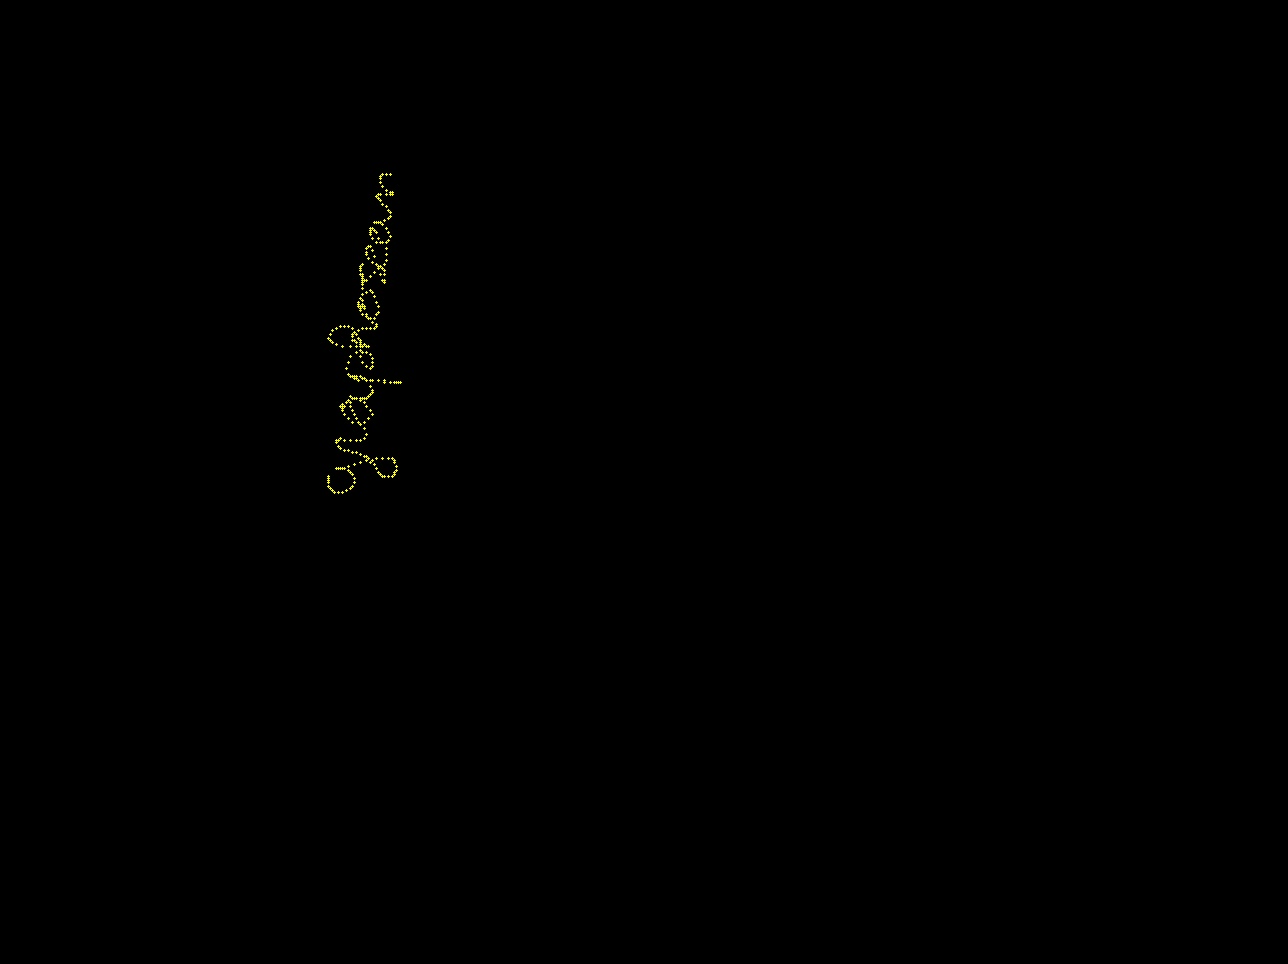
\includegraphics[width=\textwidth, height=4cm]{Modules/Picture/tracking.png}
\caption{reconnaissance avec le tracking}
\label{tracking}
\end{figure}

\begin{figure}[!h]
\centering
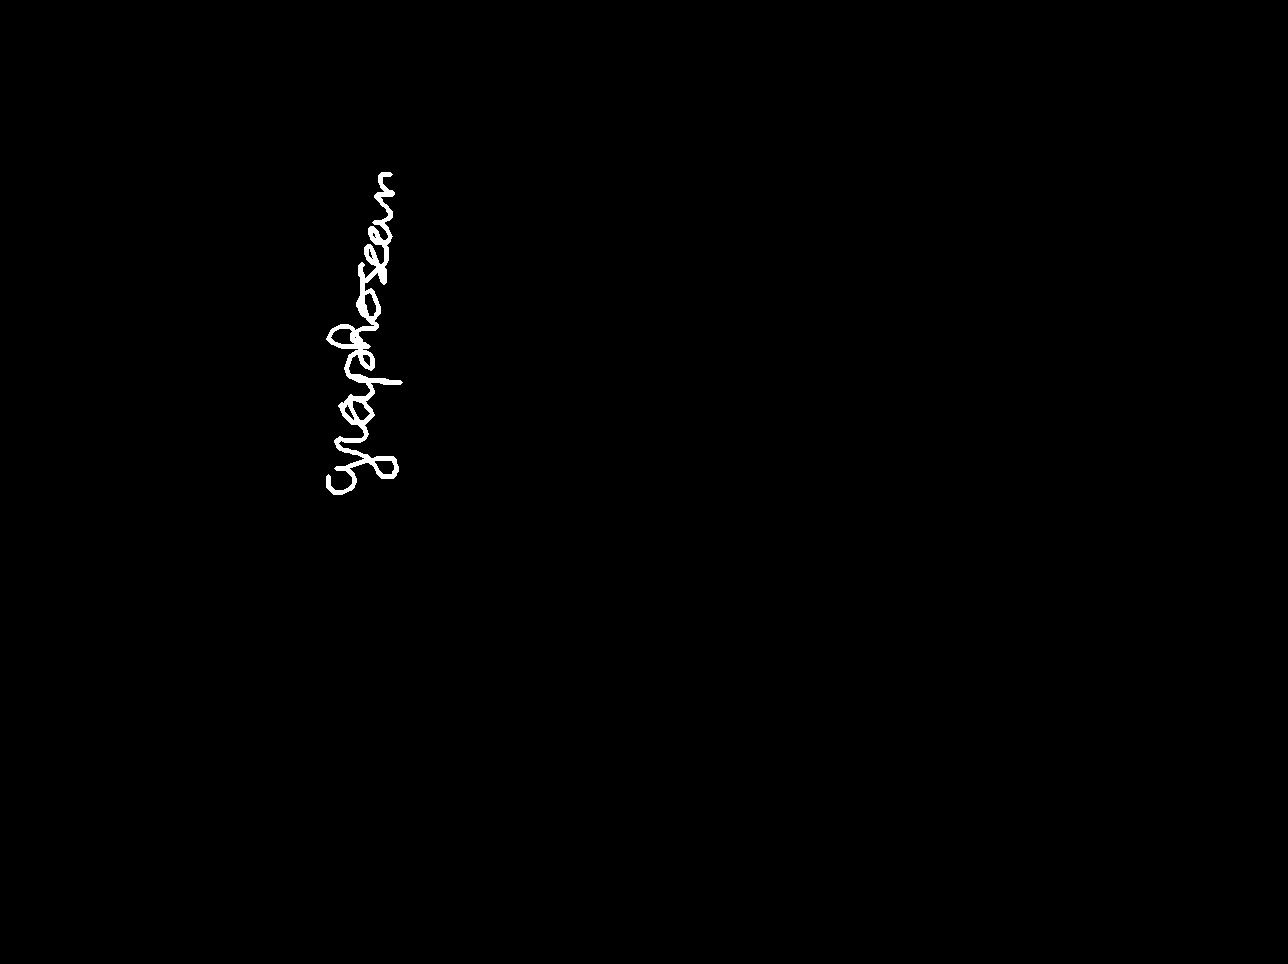
\includegraphics[width=\textwidth, height=4cm]{Modules/Picture/hog_propre.png}
\caption{HOG non nettoyé}
\label{HOGSale}
\end{figure}

\begin{figure}[!h]
\centering
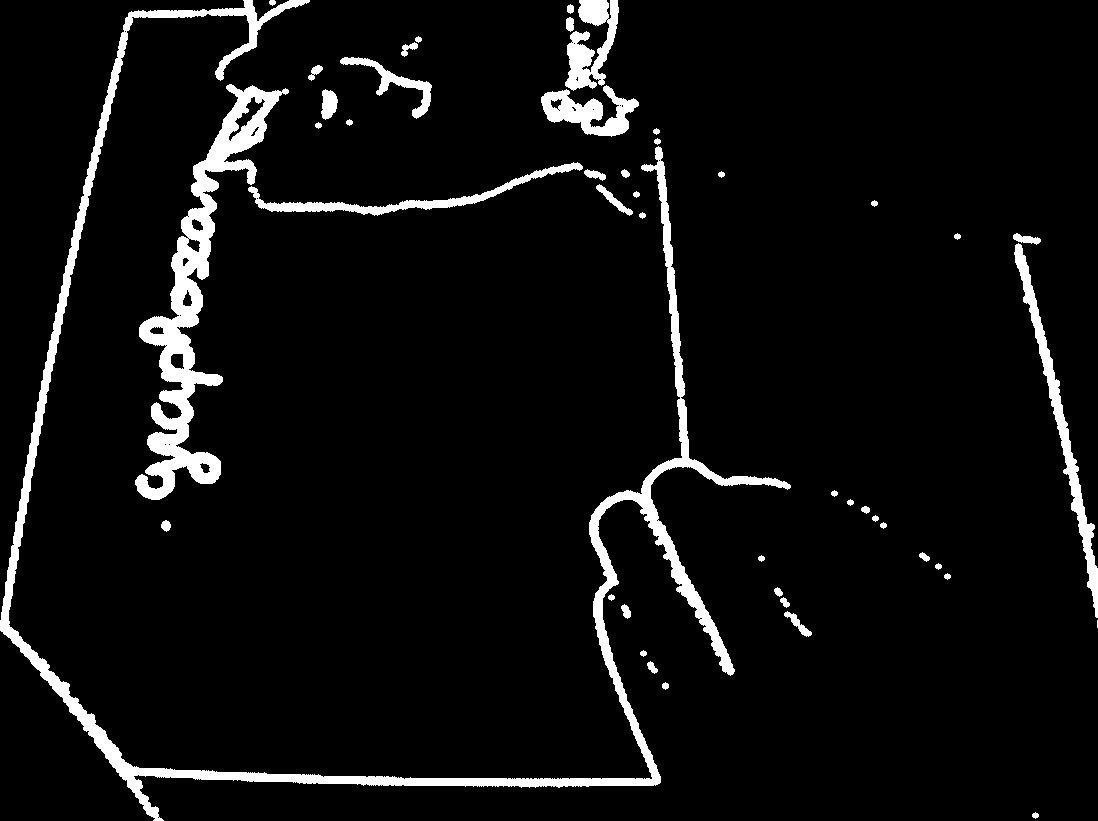
\includegraphics[width=\textwidth, height=4cm]{Modules/Picture/hog.png}
\caption{reconnaissance avec HOG}
\label{HOGPropre}
\end{figure}